\section{Modelo de TRFs por regresión regularizada}
\label{sec:modelo_regresion}

% Describir cómo se incorporan las variables al modelo de regresión EEG.
% Explicar la estrategia de construcción incremental:
% partir del mejor modelo base, agregar variables de a una,
% seleccionar las que sobreviven, luego agregar interacciones.
% Justificar la estrategia.

El objetivo principal de esta tesis es investigar si las variables extraídas del modelo nnELM tienen correlatos con la actividad neural. El análisis de la actividad cerebral durante las tareas de búsqueda visual tiene una dificultad particular: las respuestas cerebrales de fijaciones sucesivas se solapan temporalmente. La duración típica de una fijación presenta una media de 219ms, un tiempo considerablemente menor a la ventana temporal necesaria para capturar una respuesta completa, la cual se extiende a lo largo de 600ms.

Como se mencionó en la Sección \ref{sec:eeg_modelo_damian}, este marco de deconvolución lineal fue aplicado sobre el dataset HSEM por \citep{care2025}, quienes desarrollaron un modelo de TRFs por regresión regularizada para estudiar los correlatos neurales de la búsqueda híbrida. A continuación se describen sus componentes principales: la noción de TRF, la construcción de la matriz de diseño y el procedimiento de estimación.

\begin{figure}[h]
    \centering
    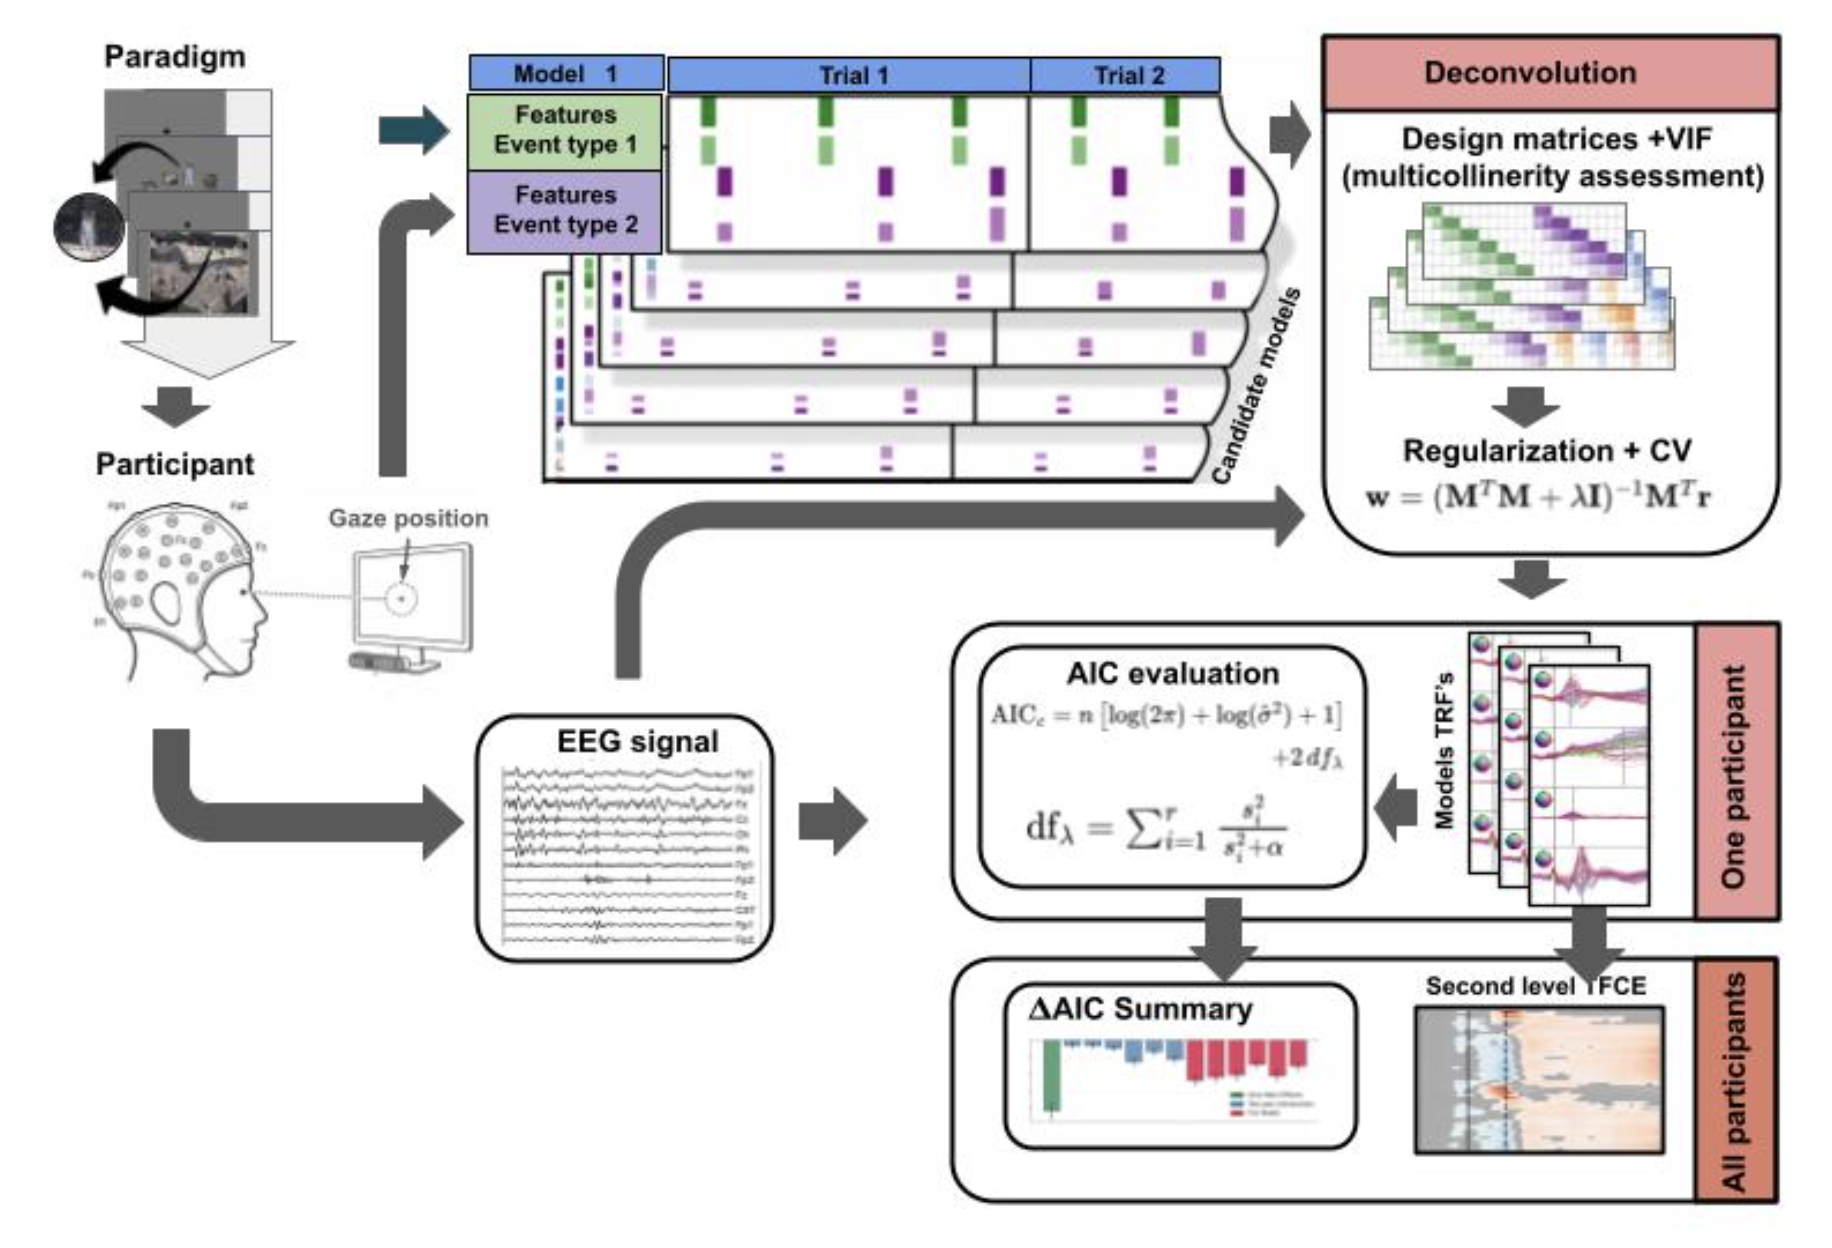
\includegraphics[width=\textwidth]{chapters/02_materiales/images/flujo_regresion.png}
    \caption{Esquema general del framework de TRFs por regresión regularizada. Extraído de \citep{care2025}.}
    \label{fig:trf_pipeline}
\end{figure}

\subsection{Temporal Response Functions (TRFs)}

Una Temporal Response Function (TRF) es la respuesta neural estimada asociada a un predictor específico en función del tiempo relativo al onset del evento.  Para cada variable del modelo, la TRF es una curva que indica cuánto varía la señal EEG en cada retardo temporal ante un cambio unitario de ese predictor: si la TRF de un predictor muestra un pico positivo a los 300ms, significa que en promedio la señal EEG aumenta 300ms después de que ese evento ocurre. De esta manera, el conjunto de TRFs del modelo describe cómo cada variable de interés modula la actividad cerebral a lo largo del tiempo.

\subsection{Construcción de matriz de diseño}

El framework de TRFs por Regresión Regularizadas representa la señal EEG de cada electrodo como una combinación lineal de las respuestas a distintos tipos de eventos. En el caso general, cada predictor $k$ contribuye con su propia respuesta $w_k(\tau)$ a lo largo de una ventana de lags. En el caso de un solo predictor $x$ con ventana de $L$ lags:

\begin{equation}
r(t) = \sum_{\tau=0}^{L} w(\tau) \cdot x(t - \tau) + \varepsilon(t)
\end{equation}

\noindent donde $r(t)$ es la señal EEG en el instante $t$; $x(t-\tau)$ es el valor del predictor $\tau$ muestras antes; $w(\tau)$ son los coeficientes que se quieren estimar (la TRF) y $\varepsilon(t)$ es el error residual. La TRF es la secuencia de coeficientes $w(\tau)$ para cada lag $\tau$.

Para cada participante se construye una matriz de diseño M que codifica, para cada muestra temporal de la señal EEG continua, qué eventos ocurrieron en una ventana temporal definida. 

Cada columna de M corresponde a un predictor desplazado en el tiempo (llamado lag). En otras palabras, para cada variable de interés y cada retardo temporal dentro de la ventana, se incluye una columna que indica el valor de esa variable en ese retardo.

\begin{table}[h]
\centering
\small
\begin{tabular}{c|ccc|ccc|ccc}
\toprule
 & \multicolumn{3}{c|}{\texttt{variable\_1} (binaria)} & \multicolumn{3}{c|}{\texttt{variable\_2} (binaria)} & \multicolumn{3}{c}{\texttt{variable\_3} (continua)} \\
 & $\tau_0$ & $\tau_1$ & $\tau_2$ & $\tau_0$ & $\tau_1$ & $\tau_2$ & $\tau_0$ & $\tau_1$ & $\tau_2$ \\
\midrule
$t_1$ & 1 & 0 & 0 & 0 & 0 & 0 & 0.8 & 0.0 & 0.0 \\
$t_2$ & 0 & 1 & 0 & 0 & 0 & 0 & 0.0 & 0.8 & 0.0 \\
$t_3$ & 0 & 0 & 1 & 1 & 0 & 0 & 0.0 & 0.0 & 0.8 \\
$t_4$ & 0 & 0 & 0 & 0 & 1 & 0 & 0.0 & 0.0 & 0.0 \\
$t_5$ & 1 & 0 & 0 & 0 & 0 & 1 & 0.3 & 0.0 & 0.0 \\
\bottomrule
\end{tabular}
\caption{Ejemplo simplificado de la matriz de diseño $\mathbf{M}$ para tres predictores y una ventana de 3 lags. Cada fila corresponde a una muestra temporal de la señal EEG continua. Las variables binarias toman valor 1 en el onset del evento y se desplazan diagonalmente con cada lag. La variable continua refleja el valor del predictor en ese retardo.}
\label{tab:matriz_disenio}
\end{table}

\subsection{Estimación ridge y selección del parámetro de regularización}

Los coeficientes del modelo (las TRFs) se estiman mediante regresión Ridge (regularización L2).

\begin{equation}
\hat{\mathbf{w}} = \arg\min_{\mathbf{w}} \left[ \sum_t \left( r(t) - \sum_{\tau} w(\tau) \cdot x(t-\tau) \right)^2 + \lambda \sum_{\tau} w(\tau)^2 \right]
\end{equation}

El primer término corresponde al error de predicción: qué tan bien el modelo explica la señal EEG observada. El segundo término es la penalización Ridge, que encoge los coeficientes hacia cero y está controlada por el parámetro $\lambda$. Esta penalización estabiliza la estimación en presencia de multicolinealidad entre predictores y previene el sobreajuste.

\subsubsection{Selección de $\lambda$}

El parámetro $\lambda$ se selecciona individualmente para cada participante y modelo mediante la técnica de \textit{cross-validation} de 10 folds. En cada iteración, el modelo se entrena sobre el 90\% de los datos para un conjunto de valores candidatos 
de $\lambda$, y se evalúa sobre el 10\% restante midiendo el coeficiente de correlación 
de Pearson entre la señal EEG predicha y la señal real. El $\lambda$ óptimo es aquel 
que maximiza la correlación promedio entre los 10 folds.